\documentclass{report}
\usepackage{tikz}
\usepackage{subcaption}

\begin{document}
\begin{figure}
\centering
  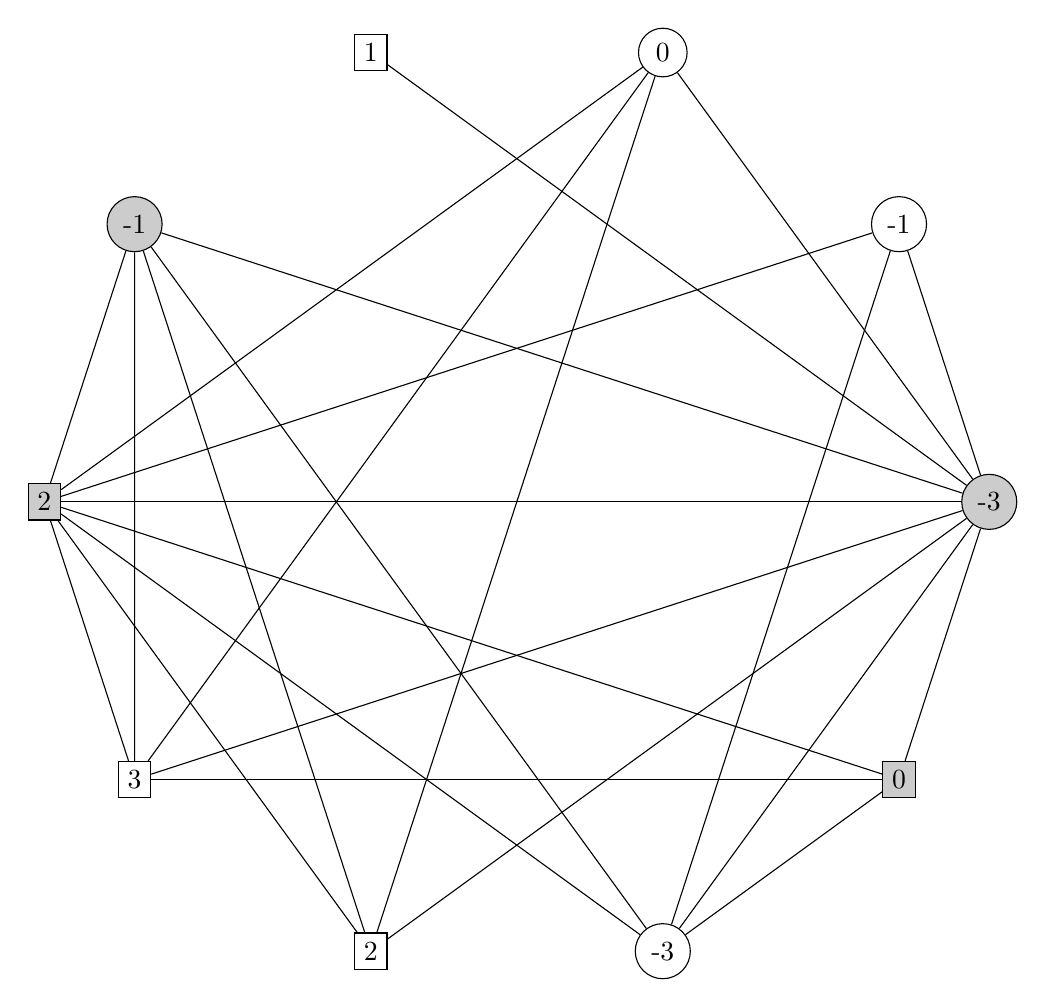
\begin{tikzpicture}[scale=3]
      \draw
        (0.0:2) node[circle, draw, fill=black!20] (0){-3}
        (36.0:2) node[circle, draw, fill=white] (1){-1}
        (72.0:2) node[circle, draw, fill=white] (2){0}
        (108.0:2) node[rectangle, draw, fill=white] (3){1}
        (144.0:2) node[circle, draw, fill=black!20] (4){-1}
        (180.0:2) node[rectangle, draw, fill=black!20] (5){2}
        (216.0:2) node[rectangle, draw, fill=white] (6){3}
        (252.0:2) node[rectangle, draw, fill=white] (7){2}
        (288.0:2) node[circle, draw, fill=white] (8){-3}
        (324.0:2) node[rectangle, draw, fill=black!20] (9){0};
      \begin{scope}[-]
        \draw (0) to (1);
        \draw (0) to (2);
        \draw (0) to (3);
        \draw (0) to (4);
        \draw (0) to (5);
        \draw (0) to (6);
        \draw (0) to (7);
        \draw (0) to (8);
        \draw (0) to (9);
        \draw (1) to (5);
        \draw (1) to (8);
        \draw (2) to (5);
        \draw (2) to (6);
        \draw (2) to (7);
        \draw (4) to (5);
        \draw (4) to (6);
        \draw (4) to (7);
        \draw (4) to (8);
        \draw (5) to (6);
        \draw (5) to (7);
        \draw (5) to (8);
        \draw (5) to (9);
        \draw (6) to (9);
        \draw (8) to (9);
      \end{scope}
    \end{tikzpicture}
\end{figure}
\end{document}